\themaM
\graphicspath{{../../S07_Horaires_et_durees/Images}}

\chapter{Horaires et durées}
\label{S07}


%%%%%%%%%%%%%%%%%%%%%%%%%%%%%%%%%%%%%%%%%%
\begin{autoeval}
   \small
   \begin{enumerate}
      \item Il effectue des calculs de durées et d'horaires.
      \item Il vérifie la cohérence des résultats du point de vue des unités pour les calculs de durées.
      \item Il effectue des conversions d'unités de durée.
   \end{enumerate}
\end{autoeval}

\begin{prerequis}
   \begin{itemize}
      \item[\com] Mener des calculs impliquant des grandeurs mesurables, exprimer les résultats dans des les unités adaptées.
      \item[\com] Exprimer et vérifier la cohérence des résultats du point de vue des unités.
   \end{itemize}
\end{prerequis}

\vfill


\begin{debat}[Débat : instruments anciens de mesure de temps et de durée]
   De tous temps on a voulu mesurer le {\bf temps} et la {\bf durée}, ci-dessous figurent quelques instruments utilisés dans des époques plus ou moins lointaines. \\
   \textcolor{B1}{\small
   \begin{tabular}{*{4}{C{3.5}}}
      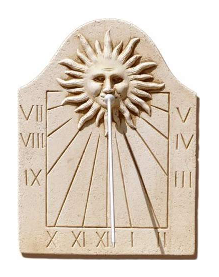
\includegraphics[width=2.8cm]{cadran}
      &
      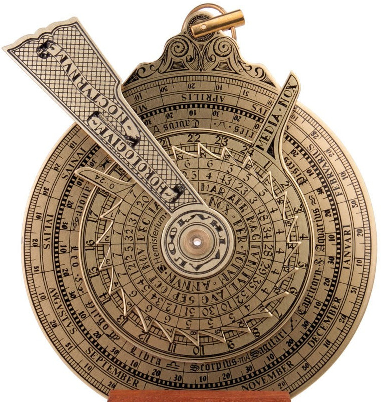
\includegraphics[width=2.8cm]{nocturlabe}
      &
      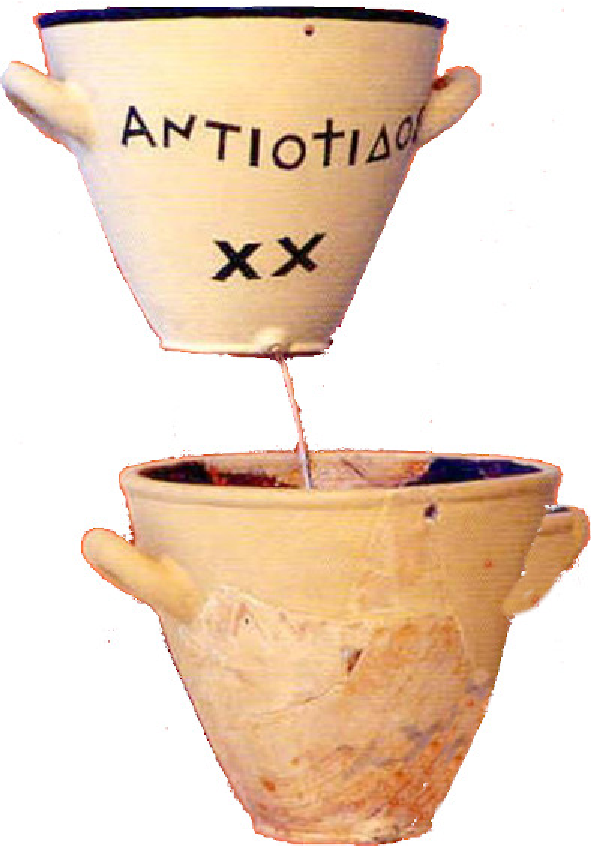
\includegraphics[width=2.8cm]{clepshydre}
      &
      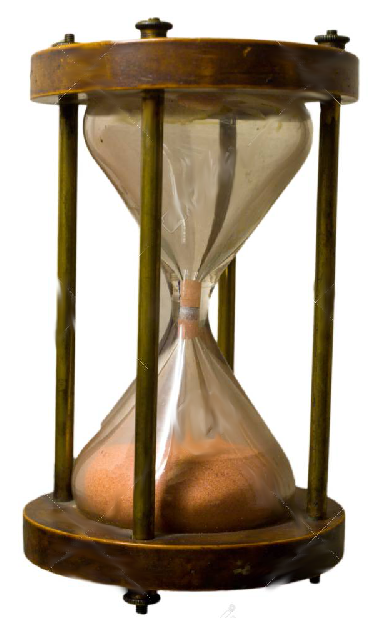
\includegraphics[width=2.8cm]{sablier} \\
      Cadran solaire & Nocturlabe & Clepsydre & Sablier \\
      1\,500 av. J.-C. & X\up{e} siècle & 1\,600 av. J.-C. & IX\up{e} siècle \\
      Heures du jour & Heures de la nuit & Durées longues (heures) & Durées courtes (minutes) \\
   \end{tabular}}
   \bigskip
   \begin{cadre}[B2][F4]
      \begin{center}
         Vidéo : \href{https://www.youtube.com/watch?v=8vMTE9U9z0U}{\bf Remettons les pendules à l'heure}, chaîne YouTube {\it C'est pas sorcier}.
      \end{center}
   \end{cadre}
\end{debat}


%%%%%%%%%%%%%%%%%%%%%%%%%%%%%%%
%%%%%%%%%%%%%%%%%%%%%%%%%%%%%%%
\activites
 
\begin{activite}[De la seconde au siècle]
   {\bf Objectif :} donner un ordre de grandeur dans le domaine des durées (plusieurs flèches peuvent arriver au même ordre de grandeur). \\
   \begin{QCM}
      Relier les durées suivantes à son ordre de grandeur.
      \begin{center}
         \begin{pspicture}(-8,-9)(8,9)
         {\psset{yunit=0.85}
            \rput(0,9){\cursive\large Le siècle}
            \rput(0,6){\cursive\large L'année}
            \rput(0,3){\cursive\large Le mois}
            \rput(0,0){\cursive\large Le jour}
            \rput(0,-3){\cursive\large L'heure}
            \rput(0,-6){\cursive\large La minute}
            \rput(0,-9){\cursive\large La seconde}
            \psdots(-1.5,-9)(-1.5,-6)(-1.5,-3)(-1.5,0)(-1.5,3)(-1.5,6)(-1.5,9)(1.5,-9)(1.5,-6)(1.5,-3)(1.5,0)(1.5,3)(1.5,6)(1.5,9)(-4,-10)(-4,-6)(-4,-2)(4,2)(4,6)(4,10)(4,-10)(4,-6)(4,-2)(-4,2)(-4,6)(-4,10)
            \rput(-6.25,-6){\parbox{3.5cm}{Temps mis par la lumière pour parcourir une distance équivalente à celle séparant la Terre et la Lune}}
            \rput(6.25,2){\parbox{3.5cm}{Durée d'un saison}}
            \rput(-6.25,2){\parbox{3.5cm}{Record du monde du \um{100}}}
            \rput(-6.25,-2){\parbox{3.5cm}{Temps de cuisson d'un \oe uf à la coque}}
            \rput(6.25,6){\parbox{3.5cm}{Intervalle entre deux battements de c\oe ur consécutifs}}
            \rput(-6.25,10){\parbox{3.5cm}{Durée d'un cycle complet de lune}}
            \rput(6.25,-6){\parbox{3.5cm}{Durée d'un film}}
            \rput(6.25,-10){\parbox{3.5cm}{Temps mis par la Terre pour faire le tour de son étoile : le Soleil}}
            \rput(6.25,10){\parbox{3.5cm}{Âge maximum atteint par un humain}}
            \rput(-6.25,6){\parbox{3.5cm}{Durée d'une grossesse}}
            \rput(6.25,-2){\parbox{3.5cm}{Durée d'un entraînement de sport}}
            \rput(-6.25,-10){\parbox{3.5cm}{Durée d'un weekend}}
            \multido{\n=-9+3}{7}{\rput(0,\n){\psframe(-1.2,-0.5)(1.2,0.5)}}}
         \end{pspicture}
      \end{center}
   \end{QCM}
\end{activite}


%%%%%%%%%%%%%%%%%%%%%%%%%%%%%%
%%%%%%%%%%%%%%%%%%%%%%%%%%%%%%
\cours 

 %%%%%%%%%%%%%
\section{Unités de temps}

Selon les situations, on indique les durées en années, mois, jours, heures, minutes, ou secondes : \\
1 siècle = 100 ans ; 1 an = 12 mois = 365/366 jours ; 1 jour = 24 heures ; 1 heure = 60 minutes = 3\,600 secondes\dots \\
Pour mesurer le temps ou une durée, on peut utiliser un cadran solaire, un sablier, une montre, un chronomètre\dots

%%%%%%%%%%%%%%%%
\section{Conversion de durées}

La seconde (s) est l'unité du système SI permettant de caractériser une durée. Contrairement aux autres unités, elle ne suit pas un système décimal, mais hexadécimal (de base 60).

\begin{methode*2*2}
   Pour convertir des heures en minutes ou des minutes en secondes ou inversement, on peut utiliser le schéma suivant : \\
   \begin{pspicture}(-1.5,-0.5)(11,3.3)
      \rnode{A}{\psframebox{durée en heures}}
      \hspace{12mm}
      \rnode{B}{\psframebox{durée en minutes}}
      \hspace{12mm}
      \rnode{C}{\psframebox{durée en secondes}}
      \nccurve[angle=90,linecolor=A1,offset=-1mm]{A}{B}
      \naput*{\textcolor{A1}{$\stackrel{\times60}{\longrightarrow}$}}
      \nbput*{\textcolor{A1}{$\stackrel{\div60}{\longleftarrow}$}}
      \nccurve[angle=90,linecolor=A1,offset=-1mm]{->}{B}{C}
      \naput*{\textcolor{A1}{$\stackrel{\times60}{\longrightarrow}$}}
      \nbput*{\textcolor{A1}{$\stackrel{\div60}{\longleftarrow}$}}
      \nccurve[angle=90,linecolor=B1]{->}{A}{C}
      \naput*{\textcolor{B1}{$\stackrel{\times3\,600}{\longrightarrow}$}}
      \nbput*{\textcolor{B1}{$\stackrel{\div3\,600}{\longleftarrow}$}}
   \end{pspicture}
   \exercice
      Convertir 170 minutes \par en heures et minutes.     
   \correction
      $170=2\times60+50$, donc \\
      $\umin{170} =\uh{2}\,\umin{50}$.
   \exercice
      Convertir \uh{1}\,\umin{25}\,\us{36} \par en secondes.
   \correction
      $\uh{1} =\us{3600}$ et $\umin{1} =\us{60}$ donc \\
      $\uh{1}\,\umin{25}\,\us{36} =\us{3600}+25\times\us{60}+\us{36} =\us{5136}$.
\end{methode*2*2}

\bigskip

Pour effectuer des additions ou soustractions de durées, on peut effectuer une opération en colonne (un peu périlleuse) ou procéder de proche en proche.
 
\begin{exemple}
\ \\ [-10mm]
  \begin{itemize}
      \item Un train part de Montpellier à \\
      8 h 48 min. La durée du trajet pour se rendre à Paris est de 3 h et 20 min. \\
      À quelle heure arrivera-t-il à Paris ?
      \item Un automobiliste part de Perpignan à 8 h 35 min et arrive à Montpellier à 10~h~20~min. Quelle est la durée de son trajet ?
   \end{itemize}
\correction
\ \\ [-8mm]
   \begin{itemize}
      \item   
      \begin{tabular}{ccccc}
         & 8 & h & 4 & 8 \\
         $+$ & 3 & h & 2 & 0 \\
         \hline
         1 & $\cancel{1}$ & h & $\cancel{6}$ & 8 \\
         \multicolumn{5}{c}{\psline{->}(0.5,0.3)(-0.5,-0.1)} \\
         1 & 2 & h & 0 & 8
      \end{tabular}
      \quad
      \begin{tabular}{p{5cm}}
        {\small on aligne les heures sous les heures, les minutes sous les minutes puis on additionne terme à terme. Si le nombre de minutes est supérieur à 60, on soustrait 60 min et on ajoute 1 h.} \\
      \end{tabular} 
      \medskip
      \item 8 h 35 $\xrightarrow{+\text{25 min}}$ 9 h 00 $\xrightarrow{+\text{1 h}}$ 10 h 00 $\xrightarrow{+\text{20 min}}$ 10 h 20. \\   
      La durée totale du trajet est de 1 h 45 min.
   \end{itemize}   
\end{exemple}

\medskip

\begin{remarque}
   attention à l'aspect hexadécimal de cette grandeur :
   \begin{itemize}
      \item lorsqu'on lit 1,5 h, cela correspond à 1 h et 0,5 h, c'est-à-dire 1h et 30 min ($0,5\times 60$ min).
      \item Inversement, 2 h 15 min ne correspond pas à 2,15 h mais à 2,25 h (15 min = $\frac{15}{60}$ h = 0,25 h).
   \end{itemize}
\end{remarque}


%%%%%%%%%%%%%%%%%%%%%%%%%%%%%%
%%%%%%%%%%%%%%%%%%%%%%%%%%%%%%
\exercicesbase

\begin{colonne*exercice}

\begin{exercice} %1
   Convertir les durées données ci-dessous en heures et minutes.
   \begin{enumerate}
      \item \uh{1,5}.
      \item \uh{2,25}.
      \item \uh{0,3}.
   \end{enumerate}
\end{exercice}

\begin{corrige}
   \ \\ [-5mm]
   \begin{enumerate}
      \item $\uh{1,5} =\blue \uh{1}\,\umin{30}$.
      \item $\uh{2,25} =\blue \uh{2}\,\umin{15}$.
      \item $\uh{0,3} =0,3\times\umin{60} =\blue \umin{18}$.
   \end{enumerate}
\end{corrige}

\bigskip


\begin{exercice} %2
   Convertir les durées données ci-dessous en heures décimales.
   \begin{enumerate}
      \item $\uh{6}\,\umin{30}$.
      \item $\uh{2}\,\umin{45}$.
      \item $\uh{8}\,\umin{33}$.
   \end{enumerate}
\end{exercice}

\begin{corrige}
   \ \\ [-5mm]
   \begin{enumerate}
      \item $\uh{6}\,\umin{30} =\blue \uh{6,5}$.
      \item $\uh{2}\,\umin{45} =\blue \uh{2,75}$. \smallskip
      \item $\uh{8}\,\umin{33} =\uh{8}+\frac{33}{60}\,\uh{} =\blue \uh{8,55}$.
   \end{enumerate}
\end{corrige}

\bigskip
 
 
\begin{exercice} %3
   Convertir les durées données ci-dessous en minutes.
   \begin{enumerate}
      \item \uh{1}\,\umin{56}.
      \item 2  j \umin{25}.
      \item 1 j \uh{20}\,\umin{3}.
   \end{enumerate}
\end{exercice}

\begin{corrige}
   \ \\ [-5mm]
   \begin{enumerate}
      \item $\uh{1}\,\umin{56} =1\times\umin{60}+\umin{56} =\blue \umin{116}$.
      \item $2\text{ j } \umin{25} =2\times24\times\umin{60}+\umin{25}$ \\
         \quad $=\umin{2880}+\umin{25} =\blue \umin{2905}$.
      \item $1\text{ j } \uh{20}\,\umin{3} =24\times\umin{60}+20\times\umin{60}+\small\umin{3}$ \\
         \quad $=\umin{1440}+\umin{1200}+\umin{3} =\blue \umin{2643}$.
   \end{enumerate}
\end{corrige}

\bigskip


\begin{exercice} %4
   Convertir les durées données ci-dessous en heures et minutes.
   \begin{enumerate}
      \item \umin{156}.
      \item \umin{296}.
      \item \umin{1603}.
   \end{enumerate}
\end{exercice}

\begin{corrige}
   \ \\ [-5mm]
   \begin{enumerate}
      \item $\umin{156} =2\times\umin{60}+\umin{36} =\blue \uh{2}\,\umin{36}$.
      \item $\umin{296} =4\times\umin{60}+\umin{56} =\blue \uh{4}\,\umin{56}$.
      \item $\umin{1603} =26\times\umin{60}+\umin{43}$ \\
         \quad $=\uh{26}\,\umin{43} =\blue 1\text{ j}\,\uh{2}\,\umin{43}$.
   \end{enumerate}
\end{corrige}

\bigskip


\begin{exercice} %5
   Effectuer les calculs suivants :
   \begin{enumerate}
      \item $\uh{3}\,\umin{45}+\uh{5}\,\umin{13}$
      \item $\uh{5}\,\umin{38}+\uh{9}\,\umin{43}$
      \item $\uh{11}\,\umin{28}-\uh{7}\,\umin{22}$
      \item $\uh{15}\,\umin{35}-\uh{9}\,\umin{49}$
   \end{enumerate}
\end{exercice}

\begin{corrige}
   \ \\ [-5mm]
   \begin{enumerate}
      \item $\uh{3}+\uh{5} =\uh{8}$ et $\umin{45}+\umin{13} =\umin{58}$ donc, $\uh{3}\,\umin{45}+\uh{5}\,\umin{13} =\blue \uh{8}\,\umin{58}$.
      \item $\uh{5}+\uh{9} =\uh{14}$ et \\
         $\umin{38}+\umin{43} =\umin{81} =\uh{1}+\umin{21}$ \\
         donc, $\uh{5}\,\umin{38}+\uh{9}\,\umin{43} =\blue \uh{15}\,\umin{21}$.
      \item $\uh{7}\,\umin{22} \quad \xrightarrow{+\umin{38}} \quad \uh{8}\,\umin{00}$ \\
         \quad\, $\uh{8}\,\umin{00} \quad \xrightarrow{+\uh{3}\;  \umin{28}} \quad \uh{11}\,\umin{28}$ \\
         $\uh{11}\,\umin{28}-\uh{7}\,\umin{22} =\uh{3}\,\umin{66} =\blue \uh{4}\,\umin{06}$.
      \item $\uh{9}\,\umin{49} \quad \xrightarrow{+\umin{11}} \quad \uh{10}\,\umin{00}$ \\
         \quad\, $\uh{10}\,\umin{00} \quad \xrightarrow{+\uh{5} \; \umin{35}} \quad \uh{15}\,\umin{35}$ \\   
         $\uh{15}\,\umin{35}-\uh{9}\,\umin{49} =\blue \uh{5}\,\umin{46}$.
   \end{enumerate}
\end{corrige}

\bigskip


\begin{exercice} %6
   Anita part à \uh{7}\,\umin{38} pour prendre le bus direction le collège Simone Veil. Elle met 6 minutes pour aller jusqu'à l'arrêt de bus, puis le trajet en bus dure 16 minutes et enfin il lui reste 4 minutes à pied. \\
   À quelle heure arrivera-t-elle au collège ?
\end{exercice}

\begin{corrige}
   Le temps de déplacement d'Anita est de \\
   $\umin{6}+\umin{16}+\umin{4} =\umin{26}$. \\
   Or, $\uh{7}\,\umin{38}+\umin{26} =\uh{7}\,\umin{64} =\uh{8}\,\umin{04}$. \\
   {\blue Anita devrait arriver au collège à \uh{8}\,\umin{04}}. \\
\end{corrige}

\bigskip


\begin{exercice} %7
   Douniya part du collège à pied à \uh{17}\,\umin{04}. Elle prévoit \umin{15}\,\us{30} pour le trajet, \umin{5} pour acheter un pain au chocolat et \umin{7} pour dire au revoir aux copines (et copains !). \\
   À quelle heure arrivera-t-elle chez elle ?
\end{exercice}

\begin{corrige}
   Le temps de déplacement de Douniya est de \\
   $\umin{15}\,\us{30}+\umin{5}+\umin{7} =\umin{27}\,\us{30}$. \\
   Or, $\uh{17}\,\umin{04}+\umin{27}\,\us{30} =\uh{17}\,\umin{31}\,\us{30}$. \\
   {\blue Douniya devrait arriver chez elle à \uh{17}\,\umin{31}\,\us{30}}. \\
\end{corrige}

\bigskip


\begin{exercice} %8
   Zayd part en promenade à \uh{9} 20. Il rentre à \uh{12}15, ne s'étant arrêté pour se reposer que lors de trois pauses de \umin{5} chacune. \\
   Pendant combien de temps a-t-il marché ?
\end{exercice}

\begin{corrige}
   $\uh{9}\,\umin{20} \quad \xrightarrow{+\umin{40}} \quad \uh{10}\,\umin{00}$ \\
   $\uh{10}\,\umin{00} \quad \xrightarrow{+\uh{2} \, \umin{15}} \quad \uh{12}\,\umin{15}$ \\
   La promenade de Zayd a duré \uh{2}\,\umin{55}. \\
   Or, il s'est arrêtée $3\times\umin{5} =\umin{15}$ donc, {\blue il a marché durant \uh{2}\,\umin{40}}. \\
\end{corrige}

\bigskip


\begin{exercice} %9
   Dans une usine, une machine met \umin{5}\,\us{26} pour fabriquer une pièce.
   \begin{enumerate}
      \item Combien de temps met-elle pour fabriquer 5 pièces ?
      \item Combien de temps met-elle pour en fabriquer 10 ?
      \item Combien de temps met-elle pour en fabriquer 20 ?
      \item Combien de temps met-elle pour en fabriquer 100 ?
      \item Combien la machine aura-t-elle fabriqué de pièces si elle fonctionne \uh{8} sans s’arrêter ?
      \item Une nouvelle machine, qui vient d’arriver à l’usine, met deux fois moins de temps pour fabriquer la même pièce. \\
      Quel temps met-elle pour fabriquer la pièce ?
   \end{enumerate}
\end{exercice}

\begin{corrige}
   \ \\ [-5mm]
   \begin{enumerate}
      \item $5\times\umin{5} =\umin{25} ; 5\times\us{26} =\us{130} =\umin{2}\,\us{10}$. \\
         $\umin{25}+\umin{2}\,\us{10} =\blue \umin{27}\,\us{10}$.
      \item $2\times(\umin{27}\,\us{10}) =\blue \umin{54}\,\us{20}$.
      \item $2\times(\umin{54}\,\us{20}) =\umin{108}\,\us{40} =\blue \uh{1}\,\umin{48}\,\us{40}$.
      \item $10\times(\umin{54}\,\us{20}) =\umin{540}\,\us{200} =\blue \uh{9}\,\umin{3}\,\us{20}$.
      \item $\uh{8} =8\times\us{3600} =\us{28800}$ et $\umin{5}\,\us{26} =5\times\us{60}+\us{26} =\us{326}$. \\
      Or, $28\,800\div326 \approx88,34$ donc, {\blue la machine aura fabriqué 88 pièces en \uh{8}}.
      \item La moitié de \umin{5} vaut \umin{2}\,\us{30} et la moitié de \us{26} vaut \us{13} donc, {\blue la machine met \umin{2}\,\us{43}}.
   \end{enumerate}
\end{corrige}

\bigskip


\begin{exercice} %10
   Résolution de problème : des robinets qui coulent. \\
   On dispose de deux robinets.
   \begin{itemize}
      \item Le premier est capable de remplir un réservoir d’eau de \ul{24} en 1 minute.
      \item Le second peut remplir ce même réservoir en 2 minutes.
   \end{itemize}
   En ouvrant les deux robinets au même moment, combien de temps faudrait-il pour remplir un jacuzzi avec \ul{1080} d’eau ? \\
   \begin{minipage}{4cm}
      \begin{enumerate}
         \item[a.] 15 min.
         \item[b.] 67,5 min.
         \item[c.] 135 min.
         \item[d.] 30 min.
      \end{enumerate}
   \end{minipage}
   \begin{minipage}{3cm}
      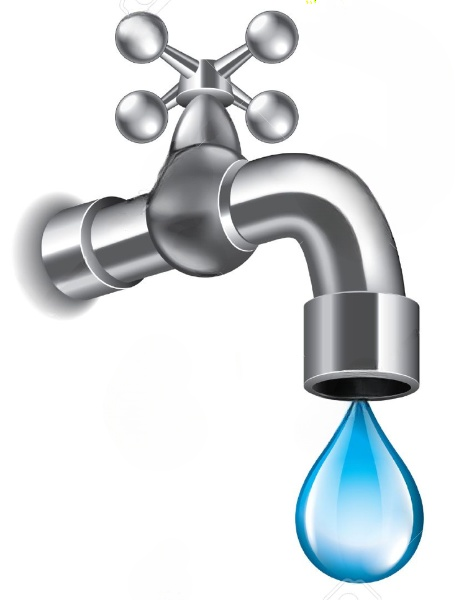
\includegraphics[width=2.5cm]{robinet}
   \end{minipage}
   
   \qquad
   \begin{minipage}{2cm}
      \qrcode{https://www.youtube.com/watch?v=8vEacS_HnNw}
   \end{minipage}
   \qquad
   \begin{minipage}{4.2cm}
      {\it Un sketch sur la résolution de problème, par Gad Elmaleh}
   \end{minipage}
\end{exercice}

\begin{corrige}
   Pour un volume à remplir, le robinet R1 met deux fois moins de temps que le robinet R2. Donc, pendant le temps total, R1 remplit deux \og unités de volume \fg{} pendant que R2 n'en remplit qu’une : \\ [1mm]
   \ModeleBarre[Largeur=2.5cm]{PowderBlue 3 {"\ul{1080}"}}{DeepSkyBlue 1 "R1" DeepSkyBlue 1 "R1" LightSkyBlue 1 "R2"} \\
   En partageant le volume total en trois parties égales, on trouve $\ul{1080}\div3 =\ul{360}$.
   R2 remplit un tiers du volume total du jacuzzi : \ul{360}. \\
   Or, $360\div12 =30$. Sachant que R2 remplit \ul{12} en \umin{1}, il remplit \ul{360} en \ul{30}. \\
   {\blue La réponse est 30 minutes (d)}. \bigskip
\end{corrige}

\end{colonne*exercice}


%%%%%%%%%%%%%%%%%%%%%%%%
%%%%%%%%%%%%%%%%%%%%%%%%
\Recreation

\newcommand{\horloge}{\psset{fillstyle=none,linecolor=lightgray,linewidth=1.5mm}
      \multido{\n=0.0+2.8,\r=2.0+2.8}{4}{\psframe(0,\n)(11,\r)} %frames
      \multido{\n=2.75+2.75}{3}{\psline(\n,0)(\n,2)}
      \multido{\n=1+1}{10}{\psline(\n,2.8)(\n,4.8)}
      \multido{\n=2.75+2.75}{3}{\psline(\n,5.6)(\n,7.6)}
      \multido{\n=2.75+2.75}{3}{\psline(\n,8.4)(\n,10.4)}
      \pscircle(5.5,12.54){1.6}
      \multido{\n=2.4+2.8}{3}{\psarc(1.25,\n){0.4}{-90}{90}
         \psarc(4.25,\n){0.4}{90}{-90}
         \psline[linewidth=3mm](1.5,\n)(4,\n)
         \psarc(6.75,\n){0.4}{-90}{90}
         \psarc(9.75,\n){0.4}{90}{-90}
         \psline[linewidth=3mm](7,\n)(9.5,\n)}
      \psarc(4.75,10.75){0.35}{-90}{90}
      \psline[linewidth=2.5mm](5.1,10.75)(5.9,10.75)
      \psarc(6.25,10.75){0.35}{90}{-90}}


\begin{enigme}[Mengenlehreuhr]
   \partie[présentation]
      La {\bf Mengenlehreuhr} (en allemand \og Horloge de la théorie du jeu \fg) ou {\bf Berlin-Uhr} (\og Horloge de Berlin \fg) est la première horloge publique au monde qui indique l'heure au moyen de champs lumineux colorés, ce qui lui a valu d'entrer dans le livre Guinness des records lors de son installation le 17 juin 1975. \\
      {\it \small Source : \href{https://en.wikipedia.org/wiki/Mengenlehreuhr}{wikipedia}}

\medskip

   \partie[recherche]
      À partir des images suivantes représentant l'horloge à différents moments de la journée, déterminer le fonctionnement de l'horloge. Par groupe, vous construirez une affiche récapitulant vos recherches. \\
      \begin{center}
      {\psset{unit=0.54}
      \begin{minipage}{6cm}  
         \begin{pspicture}(0,-1.5)(11,13.8)
            \rput(5.5,6.5){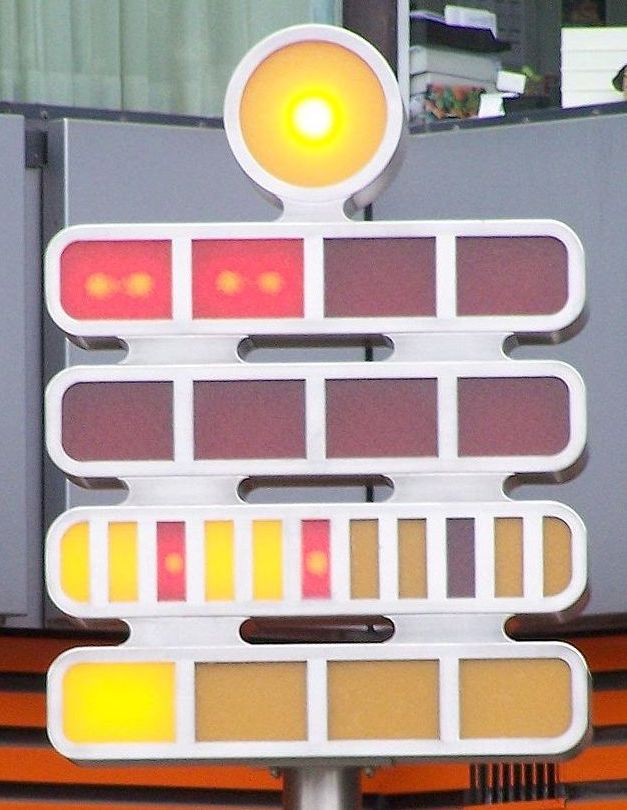
\includegraphics[width=6.7cm]{horloge_Berlin}}
         \end{pspicture}
      \end{minipage}
      \hspace{2cm}
      \begin{minipage}{6cm}  
         \begin{pspicture}(0,-1)(11,13.8)
            \psset{linecolor=yellow,fillstyle=solid,framearc=0.35}
               \psframe*(0,0)(2.75,2) %m1
               \psframe*(0,2.8)(5,4.8) %m5
               \pscircle*(5.5,12.54){1.6}
            \psset{linecolor=OrangeRed}
               \psframe*(2,2.8)(3,4.8) \psframe*(5,2.8)(6,4.8) %mi
               \psframe*(0,8.4)(5.5,10.4) %h5  
            \horloge
            \rput(5.5,-1){\large Il est 10h31}
         \end{pspicture}
      \end{minipage}
      
      \begin{minipage}{6cm}  
         \begin{pspicture}(0,-1)(11,15.5)

            \psset{linecolor=yellow,fillstyle=solid,framearc=0.35}
               \psframe*(0,0)(2.75,2) %m1
               \psframe*(0,2.8)(1,4.8) %m5
            \psset{linecolor=OrangeRed}
               \psframe*(0,5.6)(2.75,7.6) %h1
               \psframe*(0,8.4)(2.75,10.4) %h5  
            \horloge
            \rput(5.5,-1){\large Il est 6h06}
         \end{pspicture}
      \end{minipage}
      \hspace{2cm}
      \begin{minipage}{6cm}  
         \begin{pspicture}(0,-1)(11,15)
            \psset{linecolor=yellow,fillstyle=solid,framearc=0.35}
               \psframe*(0,2.8)(11,4.8) %m5
            \psset{linecolor=OrangeRed}
               \psframe*(2,2.8)(3,4.8) \psframe*(5,2.8)(6,4.8) \psframe*(8,2.8)(9,4.8) %mi
               \psframe*(0,5.6)(8.25,7.6) %h1
            \horloge
            \rput(5.5,-1){\large Il est 3h55}
         \end{pspicture}
      \end{minipage}}
      \end{center}
\end{enigme}

\begin{corrige}
   Chaque case allumée indique une durée écoulée :
   \begin{itemize}
      \item chaque case allumée de la première ligne en partant du haut représente 5 heures ;     
      \item chaque case allumée de la deuxième ligne représente 1 heure ;
      \item chaque case allumée de la troisième ligne représente 5 minutes. Les lumières rouges indiquent les quarts d’heure ;
      \item chaque case allumée de la dernière ligne représente 1 minute.
   \end{itemize}
  On additionne les durées pour obtenir l'heure.
\end{corrige}

